% \begin{figure}
%     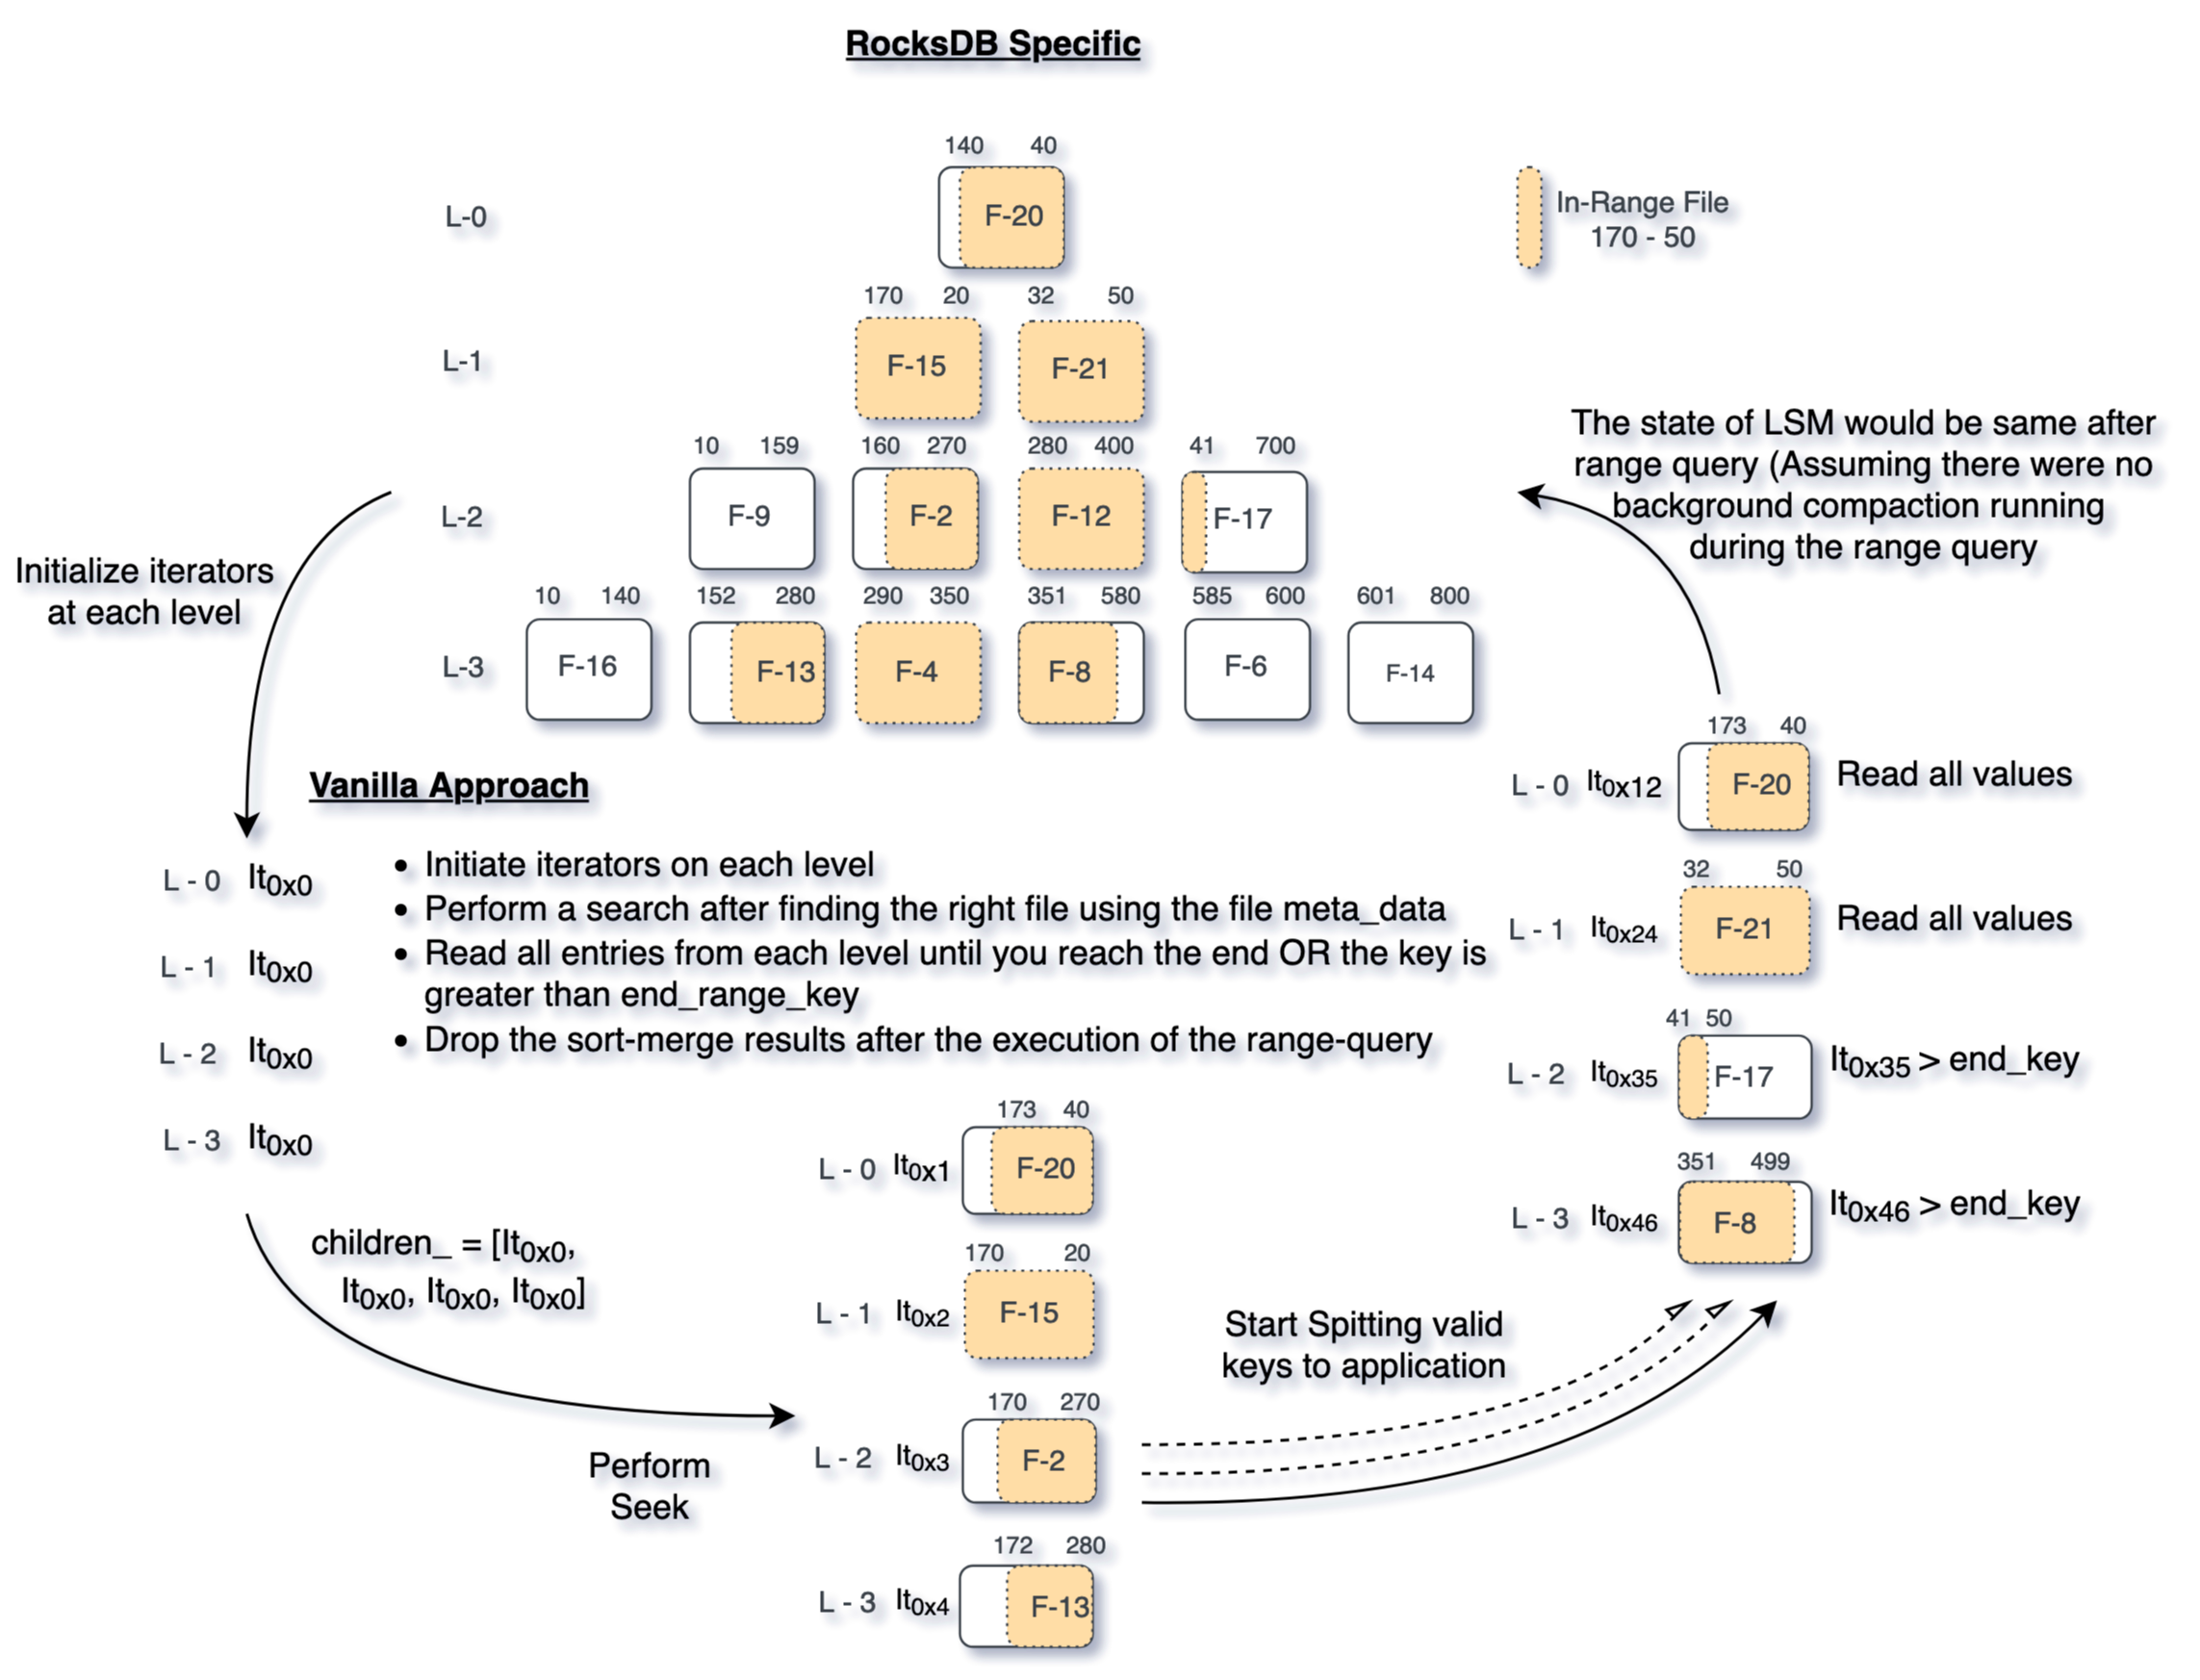
\includegraphics[scale=0.10]{Figures/Vanilla Range Query rocksdb specific.png}
%     \caption{Range query flow in lexicographically sorted files}\label{fig:rocksdb_specific_vanilla_range_query}
% \end{figure}
\begin{figure}
    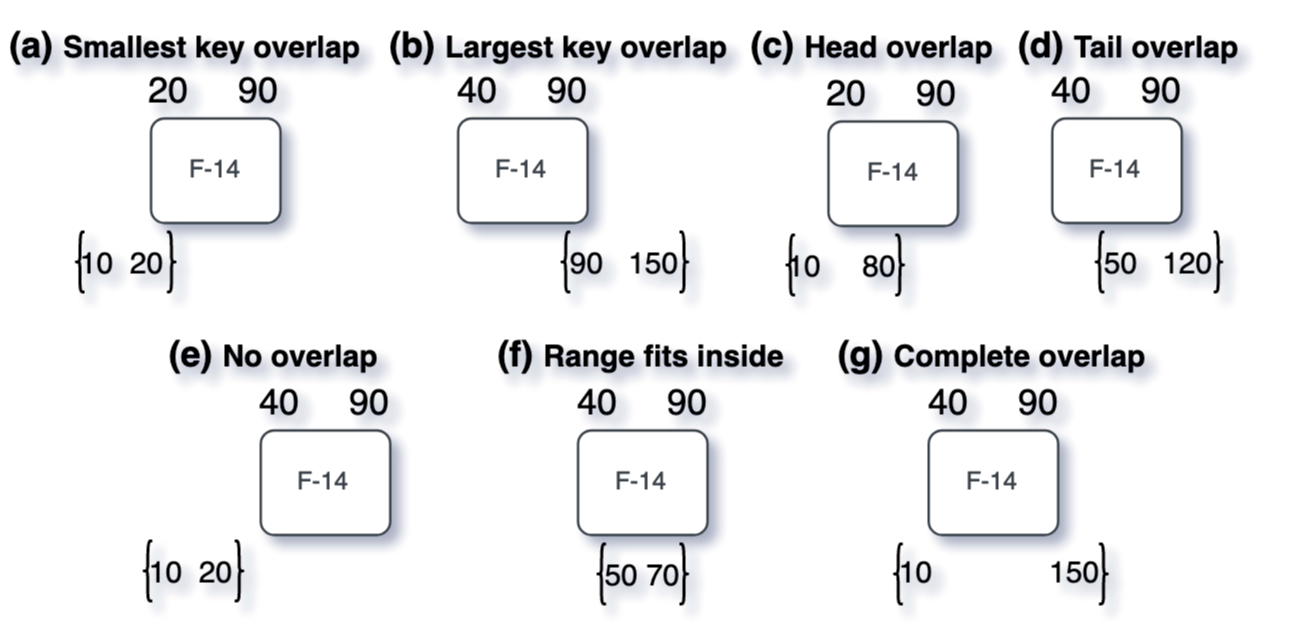
\includegraphics[scale=0.2]{Figures/File range overlaps.png}
    \caption{File range-query overlaps}\label{fig:file_range_overlaps}
\end{figure}

In the preceding background section, the compaction process (specifically, the Leveled compaction) was discussed, 
highlighting its occurrence between adjacent levels. Now, let's delve into a scenario involving an LSM tree with $N$ 
levels and a set \textit{size ratio} of 10, which is compaction triggering threshold for levels. In this context, the compaction process selects files randomly from lower 
levels based on the configured compaction policy.

Let's consider a scenario where each level shares at least one common key, which means we have $N-1$ invalid keys in our 
LSM tree. Now, envision the 
initiation of compaction from the lowest level (level 0) to the highest level, sequentially. In this process, a 
specific key would be read $N$ times and written $N$ times. This repetition arises as the key is initially read from 
level 0 and subsequently written to level 1, then read from level 1 and written to level 2, and so on. This simple 
illustration serves to demonstrate the concept of read and write amplification. However, it's important to recognize 
that in actuality, the compaction process is significantly more intricate, involving multiple files across multiple 
levels. As a result, the read and write amplification is notably higher in complex cases.

\begin{figure*}
    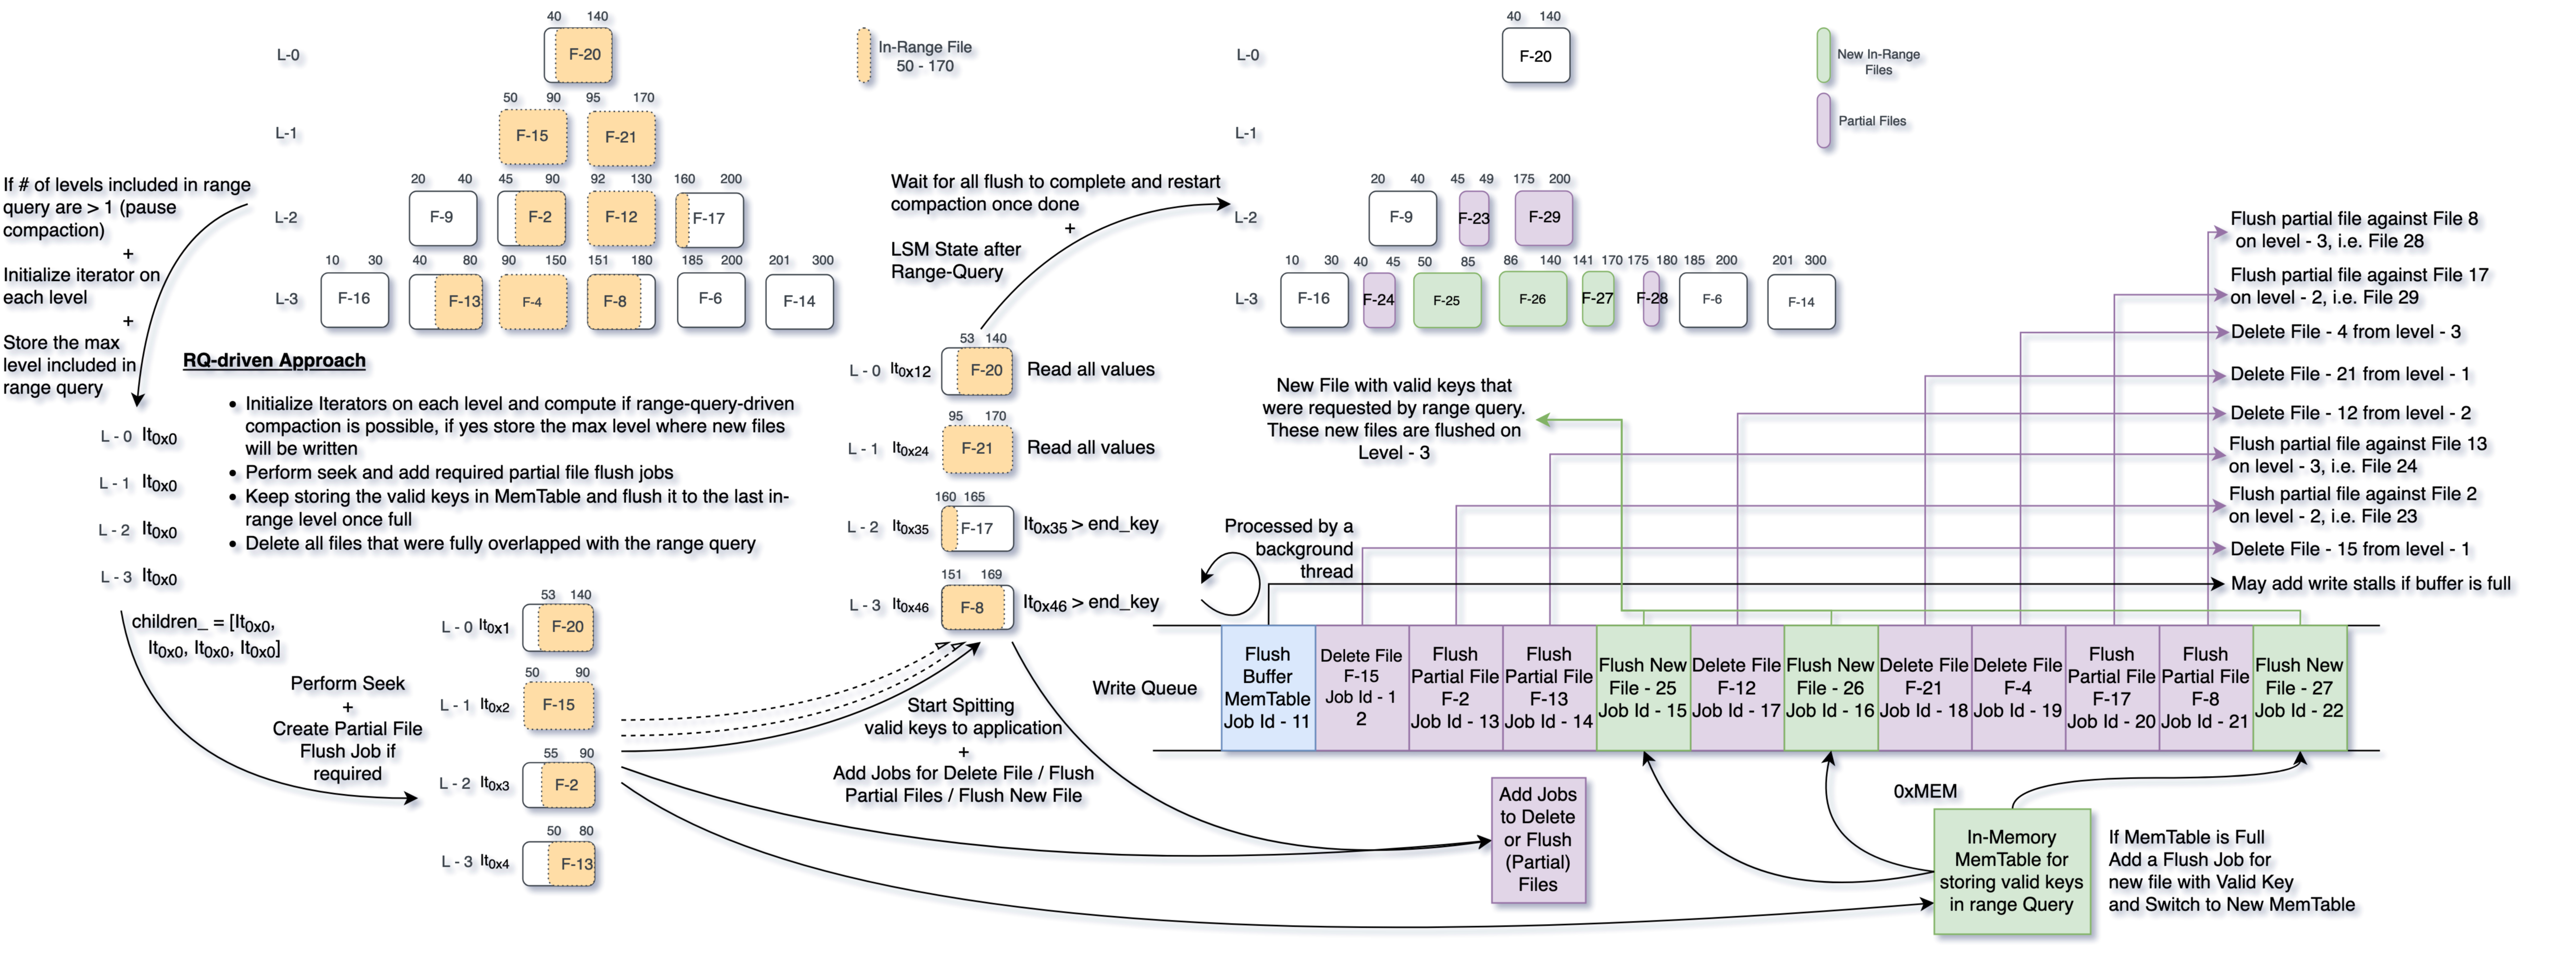
\includegraphics[scale=0.10]{Figures/RQ-driven numeric key sorting.png}
    \caption{Query-driven compaction flow in LSM}\label{fig:query-driven_compaction}
\end{figure*}

For a more tangible understanding, consider the ideal scenario where the \textit{size ratio} is 10. In this case, to 
propagate a single byte from the $i^{th}$ level to the $(i+1)^{th}$ level, a maximum of 11 bytes must be read.
Applying this principle to the earlier example, with $N$ levels each containing the same key, we effectively encounter 
the need to read and write 11 bytes a total of $N$ times due to the presence of $N$ levels sharing the common key.